% From mitthesis package
% Version: 1.10, 2025/04/27
% Documentation: https://ctan.org/pkg/mitthesis


\chapter{Introduction}

% terms:
% - workload = the bundle of endpoints/functions that are running in the same container/isolation entity
% - process = a literal linus process
% - entity = linux term: a runnable thing, either process or a cgroup that contains processes


The benefits of best effort (BE) workloads in an ideal world are clear: under
high load latency critical workloads run without impediment, but in times of low
load BE runs opportunistically and the servers can maintain high utilization. 

In order to realize these benefits, the scheduler that runs these workloads on
each machine needs to know what each workloads' priority is, and dynamically
reallocate CPUs as load changes. Linux, by far the most commmon operating system
for servers, uses \cgroups{} to group processes and know what their resource
requirements are, and schedules with these in mind. Workloads are run in an
isolation context, usually either in containers or VMs, and these rely on
\cgroups{} to implement the configured resource split.
% https://en.wikipedia.org/wiki/Usage_share_of_operating_systems
\hmng{a little awk, but I think saying the things that need to be said. Flow
could to be cleaner}

\section{The \cgroups{} interface}

\cgroups{} are a Linux construct that group processes, and apply resource
constraints on a per-group basis. This allows resource restrictions apply to the
group rather than individual processes. When processes spawn threads/new
processes, those are by default in the same group.

Users specify the resources that each group should get via interface files that
Linux exposes in a pseudo-filesystem (at \texttt{/sys/fs/cgroup}), and can move
processes into a group by writing the pid to a file there. There are many
different resource constraints that can be placed on a group, for many different
resources (\eg{} cpu, memory, i/o). There are three main interface files that
affect the cpu allocation:
\begin{enumerate}
    \item \texttt{cpu.max}: specified using two numbers: \textit{max} and \textit{period}. Linux
    enforces that the group is only allowed to use \textit{max} runtime in \textit{period} time.
    \item \texttt{cpu.weight}: a single number, in the range [1, 10000]. This
    sets the relative weight of the group. Linux broadly implements a weighted fair
    share scheduling policy, so the CPU time a group should get is defined as
    the ratio of its weight to the full weight of currently runnable groups.
    \item \texttt{cpu.idle}: 0 or 1, this sets the \textit{scheduling policy} of
    the group to be \schedidle{}.
\end{enumerate}

We discuss what exactly scheduling policies are and how they affect the
scheduler in chapter \ref{chp:sched_idle}; since the cpu.idle \cgroups{}
interface file is relatively new (added in 2021), the software discussed below
does not yet support setting this. Thus the main interface files that are used
by existing software isolation systems are \texttt{cpu.max} and
\texttt{cpu.weight}.

Given the rigid nature of the \texttt{cpu.max} interface, and the dynamic
reallocation needed to support BE workloads, we will find that all the isolation
interfaces use \texttt{cpu.weight} to splits between LC and BE tasks.

\section{How containers use \cgroups{} to dyanimically isolate BE workloads}

Containerization systems consist of two pieces: a low-level runtime, which is in
charge of actually creating and starting the containers, and a high-level
engine, which manages the containers and other metadata. Examples of low-level
runtimes include runc and crun; popular high-level engines include Docker,
Podman, containerd, and CRI-O. The low-level runtime and high-level engine
communicate via a standardized interface, specified in the Open Container
Initiative (OCI). Having a standardized interface allows different engines to
support different low-level runtimes without needing specialized code for each.

The OCI has different interfaces for different operating systems, but for Linux
specifies that \cgroups{} is used to `restrict resource usage for a container'.
Each container gets its own group, and resource restrictions/requirements are
enforced by writing the desired values to the relevant \cgroups{} interface
files. Any process or thread that is then started in the container (\ie{} group)
stays within the same group and is subject to the same restrictions. This means
that any OCI compliant container system, including all the ones listed above,
rely on \cgroups{} to restrict containers' resource usage.

Kubernetes\cite{TODO}, for example, allows users to specify cpu resource
requirements in two ways: requests and limits. Limits are directly passed on to
the \cgroups{} cpu.limit interface. Requests support the burstability required
of BE workloads, for which Kubernetes relies on \cgroups{}' \texttt{cpu.weight}
feature. BE containers are defined as containers that have no resource requests
or limits, for which Kubernetes sets the weight to the lowest weight value,
\ie{} 1.

% OCI interface
% - https://github.com/opencontainers/runtime-spec/blob/main/config-linux.md
% - https://github.com/opencontainers/runtime-spec/blob/main/spec.md

% runc
% - https://github.com/canonical/runc-app/blob/master/docs/systemd.md
% - https://github.com/opencontainers/runc/blob/main/docs/cgroup-v2.md

% crun
% - https://www.redhat.com/en/blog/introduction-crun

% containerd: 
% - https://github.com/containerd/containerd/blob/main/docs/getting-started.md 

% docker: 
% - https://dev.to/mochafreddo/understanding-docker-containers-leveraging-linux-kernels-namespaces-and-cgroups-4fkk
% - https://docs.docker.com/engine/daemon/alternative-runtimes/
% - https://docs.docker.com/engine/containers/resource_constraints/

% podman
% - https://docs.podman.io/en/latest/

% general overviews:
% - https://www.aquasec.com/blog/container-isolation-techniques/
% - https://www.aquasec.com/cloud-native-academy/container-security/container-runtime/
% - https://www.cloudraft.io/blog/container-runtimes
% - https://www.wiz.io/academy/container-runtimes



\section{How VMs use \cgroups{} to dyanimically isolate BE workloads}

We discuss KVM and Firecracker as representative examples of popular VMs.\hmng{
what other ones should I do? or is this fine}

KVM does not natively support dynamic CPU allocations between VMs. The default
interface for specifying cpu requirements is just a number of vCPUs, which is an
integer and directly defines the number of CPUs the VM will get. It is possible
to oversubscribe the vCPUs with respect to to the number of physical cores, but
it is not natively possible to control the way that KVM handles the scheduling
of VMs that share underlying cores. However, KVM does integrate with libvirt,
which allows users to specify a number of cpu `shares' for each VM. Shares are
the same thing as weight: `shares' was the \cgroups{} v1 version of what is now
cpu.weight. 1024 shares correspond to 1vCPU, and the shares a VM gets can be
less. libvirt has now upgraded to \cgroups{} v2, and although the conguration is
still called shares, libvirt relies on the \texttt{cpu.weight} interface to
enforce the shares.
% https://blog.zencoffee.org/2019/10/cpu-and-device-shares-in-libvirt
% https://libvirt.org/formatdomain.html#cpu-allocation
% https://docs.redhat.com/en/documentation/red_hat_enterprise_linux/7/html/virtualization_deployment_and_administration_guide/sect-overcommitting_with_kvm-overcommitting_virtualized_cpus
% https://nb.fedorapeople.org/cvsfedora/web/html/docs/virtualization-guide/f12/en-US/html/sect-Virtualization_Guide-Tips_and_tricks-Overcommitting_with_KVM.html
% https://www.quora.com/How-do-hypervisors-oversubscribe-the-physical-CPU-to-virtual-CPUs

Firecracker uses KVM without libvirt under the hood, but still supports VMs
having weights. It uses \cgroups{} to do this: when the jailer sets up the
environment that the VM will run in, if a weight for the VM was specified, the
jailer will create a group with that weight and put the VM inside it.
% https://github.com/firecracker-microvm/firecracker/blob/main/docs/prod-host-setup.md
% https://github.com/firecracker-microvm/firecracker/blob/a02fc1eaf18388d05feaa6f52073c7a08c8a7a75/src/jailer/src/cgroup.rs


\section{Where Linux fails}

In principle, the \texttt{cpu.weight} range of 1--10000 is large, and should
allow for BE tasks to have a negligible performance impact on LC tasks, even
during high load. However, we find that even when setting the weights of
processes to the outermost extremes, the presence of low weight (ie BE) tasks
has a large performance impact on a high-weight (ie LC) task.


\begin{figure*}[t]
    \centering
    \begin{subfigure}[t]{0.48\textwidth}
        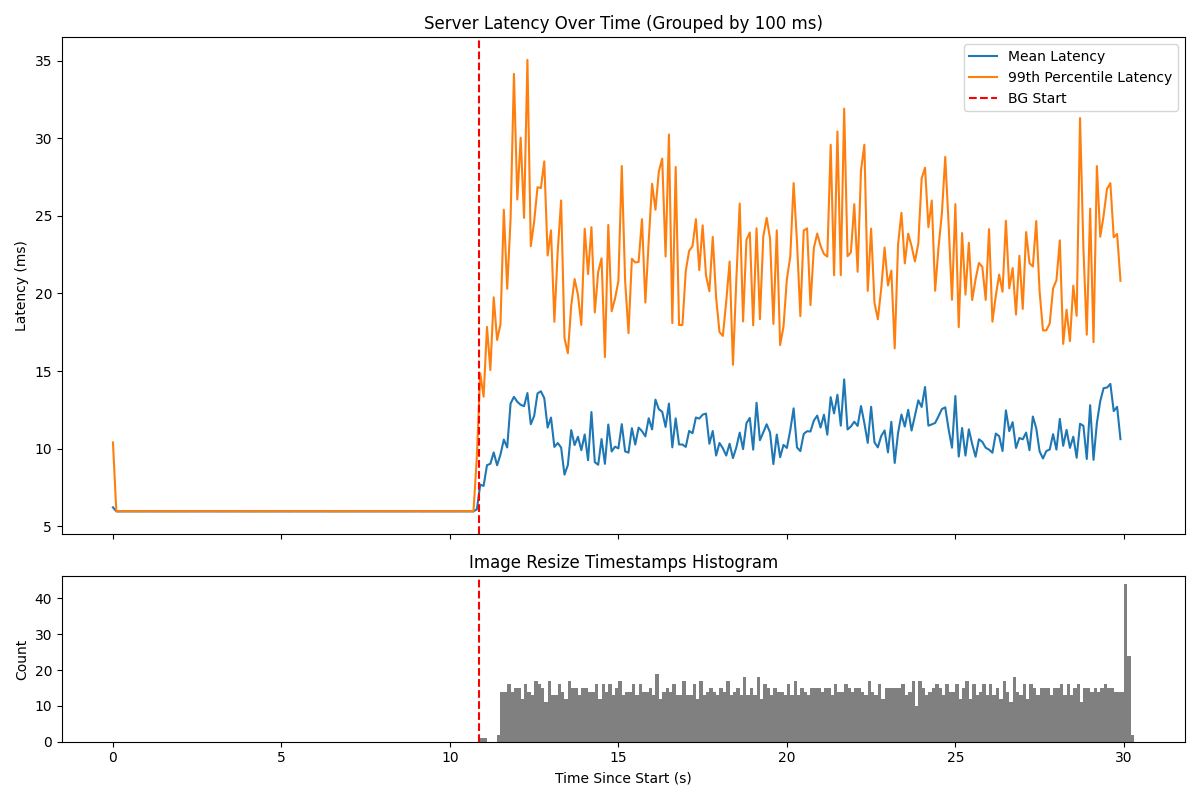
\includegraphics[width=\textwidth]{graphs/unedited-weight-low-two.png}
        \caption{Low load stetting}\label{fig:unedited-weight-low-two}
    \end{subfigure}
    \hspace{\fill}
    \begin{subfigure}[t]{0.48\textwidth}
        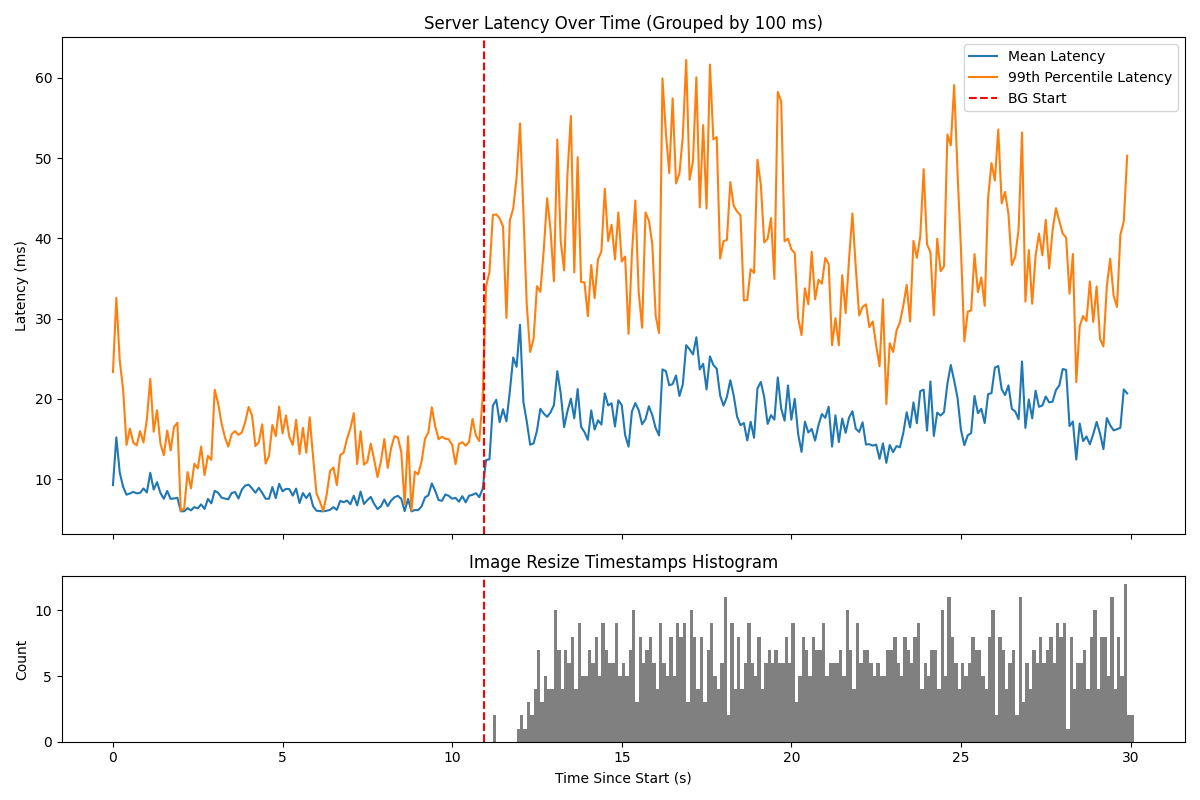
\includegraphics[width=\textwidth]{graphs/unedited-weight-high-two.png}
        \caption{High load setting}\label{fig:unedited-weight-high-two}
    \end{subfigure}
    \caption{Latencies of the server and iteration counts of the background
    tasks in different load scenarios. Note the different y axis limits. The
    upper graphs show end-to-end request latencies, and the bottom graph is a
    histogram of completed iterations of the BE tasks}\label{fig:unedited-weight}
\end{figure*}

In an experiment, we run a (LC) server that processes requests coming in from an
open loop client, running on a separate machine. The client has 100 connections
to the server, each connection creates a new server thread that reads from the
socket and synchronously processes requests in a tight loop. The server threads
run in a cgroup with the highest possible weight: 10000. The server initially
runs on an uncontended four cores, during which time the cpu utilization of the
server is around 85\%. After $\sim$10 seconds, we start two background tasks on
the same four cores, each performing an image resize job. Each background task
is in its own cgroup, which both have the lowest possible weight, 1. We then
measure the latencies experienced by the LC server, before and after starting
the background tasks. Figure~\ref{fig:unedited-weight-low-two} shows the
results. We see that mean latencies spike up from steady at just under 6ms to as
high as 13ms, and much higher for 99th percentile latencies.

With a higher baseline load for the LC server the spikes are higher,
figure~\ref{fig:unedited-weight-high-two} shows the latencies when the
utilization of the uncontended server load is around 95\%.
